\documentclass[UTF8,a4paper,12pt]{ctexart}

\usepackage{amsmath,amssymb}
\usepackage{geometry}
\usepackage{array,tabularx}
\usepackage{enumitem}
\usepackage{fancyhdr}
\usepackage{tikz}
\usepackage{lastpage}
\usepackage{xurl}
\usepackage[colorlinks=true, linkcolor=black, urlcolor=black]{hyperref}

\geometry{
  left=2.2cm,
  right=2.2cm,
  top=1.8cm,
  bottom=1.8cm
}

\setlength{\parindent}{0pt}
\setlength{\parskip}{0.5em}

\pagestyle{fancy}
\fancyhf{}
\renewcommand{\headrulewidth}{0pt}
\cfoot{\zihao{-5}第~\thepage~页~~共~\pageref{LastPage}~页}

\newcommand{\blank}[1][3cm]{\underline{\hspace{#1}}}
\newcommand{\fillblank}[2]{\underline{\makebox[#1][c]{#2}}}
\newcolumntype{C}[1]{>{\centering\arraybackslash}m{#1}}

\begin{document}

\thispagestyle{empty}

\begin{center}
    {\heiti\zihao{3} 说明}
\end{center}

\vspace{2em}

本资料由 Fishplate 整理制作。原始内容参考了一份来路不明但考证基本准确的2023级同学期末考（或是补考，来源无从考证）的影印版试卷，由衷的感谢提供试卷的John Doe同学，向勇士致敬！笔者对试卷内容进行了重新排版、整理和校对，修改了一些原试卷的错误。此外，也尽量还原原卷题目形式，但鉴于\LaTeX{}和Word文档排版方式的差异，只能做到尽量还原，请各位见谅。

\vspace{1em}

需要说明的是，本试卷共分为四个部分。卷一和卷二来源如上述所说，来源于两套来路不明的，但极大概率为2024-2025学年第二学期的试卷（2023级信通学生的考试试卷）。由于信息论考试采用半机考半笔试，机考客观题部分无从考证，只有零星的几道题目，放在了卷三。卷四来源于2018级老师哥师姐留下来的遗产，参考价值不大，但还是贴出来了。

\vspace{1em}

笔者推测大概率卷一出自2023级的补考试卷，因为根据所得的题目数推测笔试部分大概率为100分，补考很可能没有机式。卷二来源未知（推测为期末考卷）且题目缺项很多，有的题设问是笔者推测出来的。以上消息均为笔者推测，请读者自行判断！

\vspace{1em}

本文档中的参考答案由 ChatGPT 5.5 生成，限于精力，笔者目前无法逐题仔细核查。因此答案仅供复习参考，不保证完全正确。如发现题目或答案存在问题，欢迎自行修改、校对和完善。

\vspace{1em}

本试卷开源至 GitHub：\url{https://github.com/Pandamonic/CUC_2024-2025_InformationTheory_Final_Exam}，供同学们自由学习、复习和二次整理使用。如果发现有错误也欢迎大家在这里改正。

\vspace{2em}

\begin{center}

{\heiti{祝大家复习顺利，考试取得好成绩!}}

{\textbf{Per Aspera Ad Astra!}}

\vspace{1em}

{\heiti btw重要的事情说三遍：}

\vspace{1em}

{\heiti 本资料是免费的，如果你是花钱买到的，说明你被坑了！！}

{\heiti 本资料是免费的，如果你是花钱买到的，说明你被坑了！！}

{\heiti 本资料是免费的，如果你是花钱买到的，说明你被坑了！！}

\end{center}

\vfill

\begin{center}
Fishplate\\
\today
\end{center}

\newpage

\begin{center}
    {\heiti\zihao{4} 中国传媒大学}\\[0.8em]
    {\heiti\zihao{3} \fillblank{1cm}{2024}—\fillblank{1cm}{2025} 学年第\fillblank{1.1cm}{2}学期期末考试试卷（卷一）}
\end{center}

\vspace{1.8em}

\begin{tabular}{@{}p{0.51\textwidth}p{0.43\textwidth}@{}}
考试科目：\fillblank{3.8cm}{信息论与编码原理}
&
课程编号：\fillblank{3.8cm}{}
\\[1.1em]
考试班级：\fillblank{3.8cm}{23级信通学院各专业}
&
考试方式：\fillblank{3.0cm}{闭卷}
\\[-0.2em]
&
\end{tabular}

\vspace{1.2em}

\begin{center}
\renewcommand{\arraystretch}{1.55}
\begin{tabular}{|C{1.8cm}|C{1.2cm}|C{1.2cm}|C{1.2cm}|C{1.2cm}|C{1.2cm}|C{1.2cm}|C{1.8cm}|C{1.8cm}|}
\hline
题目 & 一 & 二 & 三 & 四 & 五 & 六 & 七 &总分 \\
\hline
得分 &  &  &  &  &  &  &  &  \\
\hline
\end{tabular}
\end{center}

\vspace{2.5em}

%==================== 第一题 ====================
\noindent
\begin{minipage}[t]{0.26\textwidth}
\renewcommand{\arraystretch}{1.5}
\begin{tabular}{|C{1.5cm}|C{2.3cm}|}
\hline
得分 & 评卷人 \\
\hline
\rule{0pt}{0.8cm}&  \\
\hline
\end{tabular}
\end{minipage}
\hspace{0.02\textwidth}
\begin{minipage}[t]{0.68\textwidth}
{\heiti 一、（每小题 2 分，共 20 分）概念题}

\vspace{0.25em}
（1--5 小题为判断题：判断\underline{\textbf{对错}}，并\underline{\textbf{纠正}}错误命题；6--10 小题为\underline{\textbf{填空题}}）
\end{minipage}

\vspace{0.9em}

\begin{enumerate}[label=\arabic*., leftmargin=2em, itemsep=1.45em]

\item 信道疑义度始终为正。\hfill（\qquad）

\item 信道容量只与信道的统计特性有关，而与输入信源的概率分布无关。\hfill（\qquad）

\item 对于马尔可夫信源来说，满足齐次性即可以满足平稳性。\hfill（\qquad）

\item 如果信息传输速率大于信道容量，就不存在使传输差错率任意小的信道编码。\hfill（\qquad）

\item 线性分组码的最小汉明距离等于所有码字的最小重量。\hfill（\qquad）

\item 设码符号集为 $X=\{0,1\}$，对应码字为
\[
\{0,\ 10,\ 110,\ 1110,\ 1011,\ 1101\}
\]
则该码\blank[1.5cm]唯一可译码。（填“是”或“不是”）

\item $R(D)$ 是满足 $D$ 限制下平均传送每个信源符号所需要的\blank[2cm]比特数。
它是定义域上的严格递\blank[1.5cm]函数。

\item 固定信道传输概率，平均互信息是信源概率分布的\blank[2cm]函数。

\item 二进制信源熵的最小值为\blank[2cm]，最大值为\blank[2cm]。

\item 由定长编码定理可知，对于给定信源，当信源的序列长度 $N$ 足够大时，
$\varepsilon$ 典型序列集合的概率趋于\blank[2cm]，非 $\varepsilon$ 典型序列集合的概率趋于\blank[2cm]。

\end{enumerate}

%==================== 第二题 ====================
\noindent
\begin{minipage}[t]{0.26\textwidth}
\renewcommand{\arraystretch}{1.5}
\begin{tabular}{|C{1.5cm}|C{2.3cm}|}
\hline
得分 & 评卷人 \\
\hline
\rule{0pt}{0.8cm}&  \\
\hline
\end{tabular}
\end{minipage}
\hspace{0.02\textwidth}
\begin{minipage}[t]{0.68\textwidth}
{\heiti 二、（10 分）}设某二进制码为$C=\{11100,\ 01001,\ 10010,\ 00111\}$求解：
\end{minipage}

\vspace{1.0em}

\begin{enumerate}[label=\arabic*., leftmargin=2em]
\item （2 分）该码字的最小汉明距离；
\item （3 分）假设码字等概分布，求解该码的信息传输速率；
\item （2 分）采用最小汉明距离译码准则，试问接收序列 $01100$ 和 $00100$
\item （3 分）请分析此码能够纠正几位码元的错误。
\end{enumerate}

\newpage

%==================== 第三题 ====================
\noindent
\begin{minipage}[t]{0.26\textwidth}
\renewcommand{\arraystretch}{1.5}
\begin{tabular}{|C{1.5cm}|C{2.3cm}|}
\hline
得分 & 评卷人 \\
\hline
\rule{0pt}{0.8cm}&  \\
\hline
\end{tabular}
\end{minipage}
\hspace{0.02\textwidth}
\begin{minipage}[t]{0.7\textwidth}
{\heiti 三、（16 分）}设有一信源，它在开始时以
$p(a)=0.6, p(b)=0.3, p(c)=0.1$
的概率发出 $X_1$。如果 $X_1$ 为 $a$ 时，则 $X_2$ 为
$a,b,c$ 的概率均为 $1/3$；如果 $X_1$ 为 $b$ 时，则 $X_2$ 为
$a,b,c$ 的概率均为
\end{minipage}

 $1/3$；如果 $X_1$ 为 $c$ 时，则 $X_2$ 为 $a,b$ 的概率为 $1/2$，而为 $c$ 的概率为 $0$。而且后面发出的 $X_i$ 的概率只与 $X_{i-1}$ 有关，且$p(X_i|X_{i-1})=p(X_2|X_1),i\geq 3$
\begin{enumerate}[label=\arabic*., leftmargin=2em]
\item （11 分）试画出状态转移图，并计算信源熵 $H_\infty$；
\item （2 分）求解该信源的剩余度；
\item （3 分）求解该信源达到稳态时的符号概率分布。
\end{enumerate}

\newpage

%==================== 第四题 ====================
\noindent
\begin{minipage}[t]{0.26\textwidth}
\renewcommand{\arraystretch}{1.5}
\begin{tabular}{|C{1.5cm}|C{2.3cm}|}
\hline
得分 & 评卷人 \\
\hline
\rule{0pt}{0.8cm}&  \\
\hline
\end{tabular}
\end{minipage}
\hspace{0.02\textwidth}
\begin{minipage}[t]{0.68\textwidth}
\vspace{0.25cm}
{\heiti 四、（14 分）}设离散无记忆信道的输入符号集
$X=\{0,1\}$，输出符号集 $Y=\{0,1,2\}$，信道矩阵为$P=
\begin{bmatrix}
1/2 & 1/4 & 1/4\\[0.4em]
1/4 & 1/2 & 1/4
\end{bmatrix}
$。
\end{minipage}
\vspace{0.3em}
\begin{enumerate}[label=\arabic*., leftmargin=2em]
\item （6 分）求该信道的信道容量，并求解达到信道容量时的输入分布和输出分布。
\item （8 分）若某信源输出两个等概消息 $S_1$ 和 $S_2$，现用信道输入符号集中的符号对 $S_1$ 和 $S_2$ 进行信道编码，以 $W_1=00$ 代表 $S_1$，$W_2=11$ 代表 $S_2$。试写出能使平均错误译码概率最小的译码规则，并计算平均错误译码概率。
\end{enumerate}
\newpage

%==================== 第五题（占位） ====================
\noindent
\begin{minipage}[t]{0.26\textwidth}
\renewcommand{\arraystretch}{1.5}
\begin{tabular}{|C{1.5cm}|C{2.3cm}|}
\hline
得分 & 评卷人 \\
\hline
\rule{0pt}{0.8cm}&  \\
\hline
\end{tabular}
\end{minipage}
\hspace{0.02\textwidth}
\begin{minipage}[t]{0.68\textwidth}
\vspace{0.85cm}
{\heiti 五、（空缺）}
\end{minipage}

%==================== 第六题 ====================
\noindent
\begin{minipage}[t]{0.26\textwidth}
\renewcommand{\arraystretch}{1.5}
\begin{tabular}{|C{1.5cm}|C{2.3cm}|}
\hline
得分 & 评卷人 \\
\hline
\rule{0pt}{0.8cm}&  \\
\hline
\end{tabular}
\end{minipage}
\hspace{0.02\textwidth}
\begin{minipage}[t]{0.68\textwidth}
\vspace{0.25cm}
{\heiti 六、（12 分）}已知线性分组码的生成矩阵如下：
\[
G=
\begin{bmatrix}
0&0&0&1&0&1&1\\
0&0&1&0&1&1&0\\
0&1&0&1&1&0&0\\
1&0&1&1&0&0&0
\end{bmatrix}.
\]
\end{minipage}
\begin{enumerate}[label=\arabic*., leftmargin=2em]
\item （6 分）当输入序列为 $0101000100001110$ 时，求编码器输出的\underline{\textbf{系统码}}的码序列。
\item （2 分）求系统码的监督矩阵。
\item （4 分）若接收 $B=1110001$，计算伴随式，并纠错。
\end{enumerate}

\newpage

%==================== 第七题 ====================
\noindent
\begin{minipage}[t]{0.26\textwidth}
\renewcommand{\arraystretch}{1.5}
\begin{tabular}{|C{1.5cm}|C{2.3cm}|}
\hline
得分 & 评卷人 \\
\hline
\rule{0pt}{0.8cm}&  \\
\hline
\end{tabular}
\end{minipage}
\hspace{0.02\textwidth}
\begin{minipage}[t]{0.68\textwidth}
\vspace{0.25cm}
{\heiti 七、（12 分）} $(7,3)$ 循环码的全部码字为
0000000,0010111,
0101110,0111001,1001011,1011100,1100101,1110010。
\end{minipage}
\begin{enumerate}[label=\arabic*., leftmargin=2em]
\item （6 分）写出该循环码的\underline{\textbf{标准形式}}的生成矩阵 $G$，并求监督矩阵 $H$。
\item （4 分）当信息位为 $101$ 时，写出所生成的\underline{\textbf{码多项式}}。
\item （2 分）分析该码的纠错能力。
\end{enumerate}

\newpage

\begin{center}
    {\heiti\zihao{4} 中国传媒大学}\\[0.8em]
    {\heiti\zihao{3} \fillblank{1cm}{2024}—\fillblank{1cm}{2025} 学年第\fillblank{1.1cm}{2}学期期末考试试卷（卷二）}
\end{center}

\vspace{1.8em}

\begin{tabular}{@{}p{0.51\textwidth}p{0.43\textwidth}@{}}
考试科目：\fillblank{3.8cm}{信息论与编码原理}
&
课程编号：\fillblank{3.8cm}{}
\\[1.1em]
考试班级：\fillblank{3.8cm}{23级信通学院各专业}
&
考试方式：\fillblank{3.0cm}{闭卷}
\\[-0.2em]
&
\end{tabular}

\vspace{1.2em}

\begin{center}
\renewcommand{\arraystretch}{1.55}
\begin{tabular}{|C{1.8cm}|C{1.2cm}|C{1.2cm}|C{1.2cm}|C{1.2cm}|C{1.2cm}|C{1.2cm}|C{1.8cm}|}
\hline
题目 & 一 & 二 & 三 & 四 & 五 & 六 & 总分 \\
\hline
得分 &  &  &  &  &  &  &  \\
\hline
\end{tabular}
\end{center}

\vspace{2.5em}

%==================== 卷二 第一题（空缺） ====================
\noindent
\begin{minipage}[t]{0.26\textwidth}
\renewcommand{\arraystretch}{1.5}
\begin{tabular}{|C{1.5cm}|C{2.3cm}|}
\hline
得分 & 评卷人 \\
\hline
\rule{0pt}{0.8cm}&  \\
\hline
\end{tabular}
\end{minipage}
\hspace{0.02\textwidth}
\begin{minipage}[t]{0.68\textwidth}
{\heiti 一、（空缺）}
\end{minipage}

%==================== 卷二 第二题 ====================
\noindent
\begin{minipage}[t]{0.26\textwidth}
\renewcommand{\arraystretch}{1.5}
\begin{tabular}{|C{1.5cm}|C{2.3cm}|}
\hline
得分 & 评卷人 \\
\hline
\rule{0pt}{0.8cm}&  \\
\hline
\end{tabular}
\end{minipage}
\hspace{0.02\textwidth}
\begin{minipage}[t]{0.68\textwidth}
{\heiti 二、（15 分）简答题。}

1.（10 分）一帧电视图像由 $20$ 万个像素组成，一个像素取 $256$ 个可辨别的亮度电平。假设每个像素的亮度电平均以等概率出现，实时传送电视图像，每秒发送 $25$ 帧图像。
\end{minipage}
\begin{enumerate}[label=（\arabic*）, leftmargin=2.5em]
\item（4 分）求平均每帧图像携带的信息量；
\item（6 分）如果信号与噪声的平均功率比值为 $30\,\mathrm{dB}$，则传送电视信号所需的带宽为多少？
\end{enumerate}

\newpage
2.（5 分）请补全费诺不等式：
\[
H(X|Y)\ \blank[1.2cm]\ H(P_E)+P_E\log(r-1),
\]
并写出其物理意义。

\vspace{13.0 cm}

%==================== 卷二 第三题（空缺） ====================
\noindent
\begin{minipage}[t]{0.26\textwidth}
\renewcommand{\arraystretch}{1.5}
\begin{tabular}{|C{1.5cm}|C{2.3cm}|}
\hline
得分 & 评卷人 \\
\hline
\rule{0pt}{0.8cm}&  \\
\hline
\end{tabular}
\end{minipage}
\hspace{0.02\textwidth}
\begin{minipage}[t]{0.68\textwidth}
{\heiti 三、（空缺）}
\end{minipage}

\vspace{2.0em}

%==================== 卷二 第四题（空缺） ====================
\noindent
\begin{minipage}[t]{0.26\textwidth}
\renewcommand{\arraystretch}{1.5}
\begin{tabular}{|C{1.5cm}|C{2.3cm}|}
\hline
得分 & 评卷人 \\
\hline
\rule{0pt}{0.8cm}&  \\
\hline
\end{tabular}
\end{minipage}
\hspace{0.02\textwidth}
\begin{minipage}[t]{0.68\textwidth}
{\heiti 四、（空缺）}
\end{minipage}

\vspace{2.0em}

%==================== 卷二 第五题（空缺） ====================
\noindent
\begin{minipage}[t]{0.26\textwidth}
\renewcommand{\arraystretch}{1.5}
\begin{tabular}{|C{1.5cm}|C{2.3cm}|}
\hline
得分 & 评卷人 \\
\hline
\rule{0pt}{0.8cm}&  \\
\hline
\end{tabular}
\end{minipage}
\hspace{0.02\textwidth}
\begin{minipage}[t]{0.68\textwidth}
{\heiti 五、（空缺）}
\end{minipage}

\newpage

%==================== 卷二 第六题 ====================
\noindent
\begin{minipage}[t]{0.26\textwidth}
\renewcommand{\arraystretch}{1.5}
\begin{tabular}{|C{1.5cm}|C{2.3cm}|}
\hline
得分 & 评卷人 \\
\hline
\rule{0pt}{0.8cm}&  \\
\hline
\end{tabular}

\vspace{1.0em}

\begin{center}
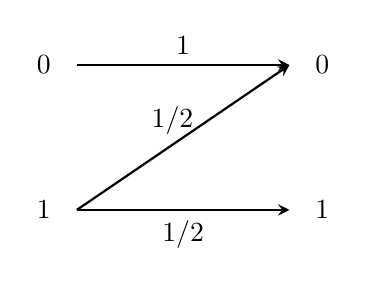
\begin{tikzpicture}[>=stealth, thick, xscale=1.0, yscale=1.15]
    % 左侧输入
    \node[left] at (0,1.8) {$0$};
    \node[left] at (0,0.2) {$1$};

    % 右侧输出
    \node[right] at (3.1,1.8) {$0$};
    \node[right] at (3.1,0.2) {$1$};

    % 三条转移线
    \draw[->] (0.2,1.8) -- (2.9,1.8) node[midway, above] {$1$};
    \draw[->] (0.2,0.2) -- (2.9,1.8) node[pos=0.45, above] {$1/2$};
    \draw[->] (0.2,0.2) -- (2.9,0.2) node[midway, below] {$1/2$};
\end{tikzpicture}
\end{center}
\end{minipage}
\hspace{0.02\textwidth}
\begin{minipage}[t]{0.68\textwidth}
{\heiti 六、（16 分）}将\underline{\textbf{两个}}如图所示的信道\underline{\textbf{级联}}，其中，$X$ 为级联信道的输入且 $0,1$ 等概，$Z$ 为级联信道的输出。

\vspace{0.8em}

\begin{enumerate}[label=\arabic*., leftmargin=2em]

\item （7 分）求级联\underline{\textbf{级联信道}}的平均互信息 $I(X;Z)$。

\item （3 分）该\underline{\textbf{级联信道}}以 $1000$ 个二元符号/秒的速率传输输入符号。请分析 $10$ 秒钟是否可以将 $10000$ 个二元符号所含的信息量全部传送完。

\end{enumerate}
\end{minipage}


\begin{enumerate}[label=\arabic*., leftmargin=2em, start=3]

\item （3 分）现对级联信道的输入符号进行简单重复编码，即以
$W_1=000$ 代表 $0$，$W_2=111$ 代表 $1$。试写出在级联信道最终输出端能使平均错误译码概率最小的译码规则，并计算平均错误译码概率。

\item （3 分）当有 $n$ 个如图所示的信道\underline{\textbf{级联}}，尝试给出此时信道转移矩阵的一般表达式 $P^n$（不用证明）；当 $n$ 趋于无穷大时，求该信道的信道容量。

\end{enumerate}

\newpage

\newpage

\begin{center}
    {\heiti\zihao{3} 2024--2025 学年第二学期}\\[0.5em]
    {\heiti\zihao{3} 信息论与编码原理期末考试试卷（卷三）}\\[0.5em]
    {\heiti\zihao{4} 部分客观题整理}
\end{center}

\vspace{1em}

\noindent
客观题共 20 道，每题 2 分。以下为目前收集到的部分客观题。由于原始材料不完整，16--20 题暂缺，后续可继续补充。

\vspace{1em}

\begin{enumerate}[label=\arabic*., leftmargin=2em, itemsep=1.4em]

\item 对于已给 $(n,k)$ 线性分组码，伴随式数目与可纠正数量 $u$ 的关系为：
\[
2^{n-k}\ \blank[1.2cm]\ \sum_{i=0}^{u} C_n^i
\]

\begin{tabular}{@{}p{0.22\textwidth}p{0.22\textwidth}p{0.22\textwidth}p{0.22\textwidth}@{}}
A. $>$ & B. $<$ & C. $\geq$ & D. $\leq$
\end{tabular}

\item $(n,k)$ 循环码的非全零码字中连 $0$ 的个数最多只能有\blank[1.5cm]位。

\begin{tabular}{@{}p{0.22\textwidth}p{0.22\textwidth}p{0.22\textwidth}p{0.22\textwidth}@{}}
A. $n-k$ & B. $k$ & C. $n-1$ & D. $k-1$
\end{tabular}

\item 以下关于信道编译码的描述中正确的有：（多选题）

\begin{enumerate}[label=\Alph*. , leftmargin=2em, itemsep=0.4em]
\item 信道编码是利用相关性来检测和纠正传输过程中产生的差错。
\item 信道译码是在接收到码符号序列后，按照与信道编码器相同的数学规律，检查并纠正错误，尽量还原符号序列。
\item 信道编码是按照一定的规则给信源编码后的码符号序列增加一些冗余信息，因而会降低通信的有效性。
\item 信道编码和信道译码是匹配的，因此没有信道编码，则无需信道译码。
\end{enumerate}

\item 由于干扰和噪声的存在，有噪无损信道无法实现端到端的无差错传输。

\begin{tabular}{@{}p{0.22\textwidth}p{0.22\textwidth}@{}}
A. 正确 & B. 错误
\end{tabular}

\item 错误译码概率与信道的统计特性有关，也与译码规则有关。

\begin{tabular}{@{}p{0.22\textwidth}p{0.22\textwidth}@{}}
A. 正确 & B. 错误
\end{tabular}

\item 已知维拉图中 $H(X)$ 表示为两个圆相交时的左边部分和相交部分的和，$H(Y)$ 表示为右边部分和相交部分的和，则 $H(Y|X)$ 表示为：

\begin{center}
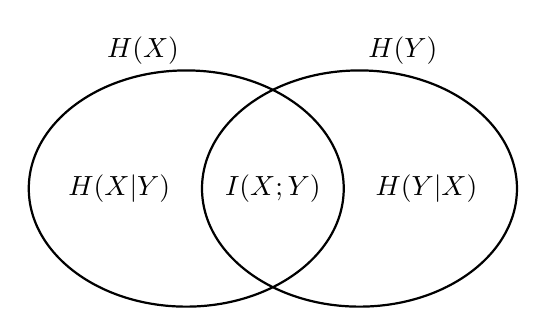
\begin{tikzpicture}[scale=1.0]
    % 两个椭圆
    \draw[thick] (0,0) ellipse (2cm and 1.5cm);
    \draw[thick] (2.2,0) ellipse (2cm and 1.5cm);

    % 上方标签
    \node at (-0.55,1.75) {$H(X)$};
    \node at (2.75,1.75) {$H(Y)$};

    % 内部标签
    \node at (-0.85,0) {$H(X|Y)$};
    \node at (1.1,0) {$I(X;Y)$};
    \node at (3.05,0) {$H(Y|X)$};
\end{tikzpicture}

图：信息维拉图
\end{center}

\begin{enumerate}[label=\Alph*. , leftmargin=2em, itemsep=0.4em]
\item 两个圆相交时的左边部分
\item 全部部分
\item 右边部分
\item 相交部分
\end{enumerate}

\item 已知信道的输入是随机变量 $X$，输出是随机变量 $Y$，噪声熵用以下函数表示：

\begin{tabular}{@{}p{0.22\textwidth}p{0.22\textwidth}p{0.22\textwidth}p{0.22\textwidth}@{}}
A. $H(Y|X)$ & B. $H(X|Y)$ & C. $I(X;Y)$ & D. $H(Y)$
\end{tabular}

\item 离散信道相关的所有概率（边缘概率、条件概率和联合概率）都可由下面选项中的哪两种概率表示？

\begin{enumerate}[label=\Alph*. , leftmargin=2em, itemsep=0.4em]
\item 信道输入概率 $p(x_i)$ 和信道转移概率 $p(y_j|x_i)$
\item 信道输入概率 $p(x_i)$ 和后验概率 $p(x_i|y_j)$
\item 信道输入概率 $p(x_i)$ 和输出概率 $p(y_j)$
\item 信道转移概率 $p(y_j|x_i)$ 和后验概率 $p(x_i|y_j)$
\end{enumerate}

\item 离散级联信道如下图所示：
\[
X\longrightarrow \text{信道 I}\longrightarrow Y\longrightarrow \text{信道 II}\longrightarrow Z
\]
$X,Y,Z$ 构成马尔可夫链。则：
\[
I(XY;Z)\ \blank[1.2cm]\ I(Y;Z),
\]
\[
I(X;Z)\ \blank[1.2cm]\ I(Y;Z),
\]
\[
P_{Z|X}\ \blank[1.2cm]\ P_{Y|X}P_{Z|Y}.
\]
依次应是：

\begin{enumerate}[label=\Alph*. , leftmargin=2em, itemsep=0.4em]
\item 大于等于，大于，小于
\item 等于，小于等于，等于
\item 小于，等于，大于
\item 小于等于，大于，等于
\end{enumerate}

\item 互信息的计算公式，不正确的是：（多选题）

\begin{enumerate}[label=\Alph*. , leftmargin=2em, itemsep=0.4em]
\item $I(x_i;y_j)=I(y_j)-I(y_j|x_i)$
\item $I(x_i;y_j)=I(x_i)-I(y_j|x_i)$
\item $I(x_i;y_j)=I(y_j)-I(x_i|y_j)$
\item $I(x_i;y_j)=I(x_iy_j)-I(x_i)-I(y_j)$
\end{enumerate}

\item 一离散信源有 $16$ 个符号，该信源的最大熵等于多少 $\mathrm{bit/}$符号？

\begin{tabular}{@{}p{0.22\textwidth}p{0.22\textwidth}p{0.22\textwidth}p{0.22\textwidth}@{}}
A. $2$ & B. $4$ & C. $6$ & D. $8$
\end{tabular}

\item 条件熵 $H(Y|X)$ 计算错误的公式是：

\begin{enumerate}[label=\Alph*. , leftmargin=2em, itemsep=0.4em]
\item $\displaystyle H(Y|X)=-\sum_i\sum_j p(y_j|x_i)\log p(y_j|x_i)$

\item $\displaystyle H(Y|X)=-\sum_i\sum_j p(x_i y_j)\log p(y_j|x_i)$

\item $\displaystyle H(Y|X)=H(XY)-H(X)$

\item $\displaystyle H(Y|X)=H(Y)-H(X)+H(X|Y)$
\end{enumerate}

\item 各维联合概率分布均与时间起点无关的信号称为平稳离散信源。

\begin{tabular}{@{}p{0.22\textwidth}p{0.22\textwidth}@{}}
A. 正确 & B. 错误
\end{tabular}

\item 对于时齐马尔可夫信源来说，极限熵不一定存在，还必须满足遍历性条件。

\begin{tabular}{@{}p{0.22\textwidth}p{0.22\textwidth}@{}}
A. 正确 & B. 错误
\end{tabular}

\item $I(X;X)=0$。

\begin{tabular}{@{}p{0.22\textwidth}p{0.22\textwidth}@{}}
A. 正确 & B. 错误
\end{tabular}

\vspace{5em}

\textbf{后面空缺。}

\end{enumerate}

\newpage

\begin{center}
    {\heiti\zihao{3} 2017--2018 学年第二学期？}\\[0.5em]
    {\heiti\zihao{3} 信息论与编码原理期末考试试卷（卷四）}\\[0.5em]
    {\heiti\zihao{4} 旧卷题目整理}
\end{center}

\vspace{1em}

\noindent
说明：本卷来源较早，题目顺序、题号和部分题干存在缺失，以下内容为根据现有材料整理得到的版本，笔者做了一些语序调整。

\vspace{1em}

%==================== 第一题 ====================

\noindent
{\heiti 一、判断与简答题}

\vspace{0.5em}

\begin{enumerate}[label=\arabic*., leftmargin=2em, itemsep=7em]

\item （空缺）

\item 对于齐次马尔可夫信源，无论初始概率分布如何，最终总会达到平稳。

\item 判断下列式子，若正确写出下式的含义，若不正确请说明理由并改正：
\[
I(X_1X_2\cdots X_N;Y)
=\sum_{i=1}^{N} I(X_i;Y|X_1X_2\cdots X_{i-1}).
\]

\item 请描述平均互信息的上凸函数性质，并以二进制对称信道为例画图说明其物理意义。

\item 请说明什么是数据处理定理？当我们在处理数据时，如何获取更多关于源数据的信息量？

\item 香农第二定理指出“高效率、高可靠性”信道编码的存在性，以及存在这种信道编码的必要条件。
其中，“高效率”是指\blank[4cm]；
“高可靠性”是指\blank[4cm]；
存在这种信道编码的必要条件是\blank[5cm]。

\end{enumerate}
%==================== 第二题 ====================

\vspace{1em}

\noindent
{\heiti 二、}有一离散无记忆信源 $X=\{0,1,2\}$，其概率分布为
$P(0)=\dfrac14,\ P(1)=\dfrac14,\ P(2)=\dfrac12$。
设计两个独立实验去观察它，其结果分别为 $Y_1=\{0,1\}$，$Y_2=\{0,1\}$。
已知条件概率如下表所示：

\begin{center}
\renewcommand{\arraystretch}{1.35}
\begin{tabular}{c|cc}
$P(Y_1|X)$ & $Y_1=0$ & $Y_1=1$\\
\hline
$X=0$ & $1$ & $0$\\
$X=1$ & $0$ & $1$\\
$X=2$ & $\dfrac12$ & $\dfrac12$
\end{tabular}
\qquad
\begin{tabular}{c|cc}
$P(Y_2|X)$ & $Y_2=0$ & $Y_2=1$\\
\hline
$X=0$ & $1$ & $0$\\
$X=1$ & $1$ & $0$\\
$X=2$ & $0$ & $1$
\end{tabular}
\end{center}

\begin{enumerate}[label=\arabic*., leftmargin=2em, itemsep=0.8em]
\item 求 $I(X;Y_1)$、$I(X;Y_2)$，并判断哪一个实验好些。
\item 求 $I(X;Y_1Y_2)$ 和 $I(X;Y_2|Y_1)$，并解释它们的含义。
\end{enumerate}

\newpage


%==================== 第三题 ====================

\vspace{1em}

\noindent
{\heiti 三、}观察长度为 $N$ 的二进制数据序列。

\vspace{0.5em}

\begin{enumerate}[label=\arabic*., leftmargin=2em, itemsep=1.0em]

\item 假定该数据序列符号前后之间没有关联，且 $P(0)=0.45,\ P(1)=0.55$。
求此时的熵 $H(X)$。

\item 将该序列视为二阶马尔可夫信源，条件概率分布为：

\begin{center}
\renewcommand{\arraystretch}{1.35}
\begin{tabular}{ll}
$P(0|00)=0.5,$ & $P(1|00)=0.5,$\\
$P(0|01)=0.8,$ & $P(1|01)=0.2,$\\
$P(0|10)=0.2,$ & $P(1|10)=0.8,$\\
$P(0|11)=0.5,$ & $P(1|11)=0.5.$
\end{tabular}
\end{center}

试计算此时的信源熵 $H_\infty$。该数据序列中大约有多少个 $0$？

\item 比较（1）和（2）中信源的剩余度，并说明其物理意义。

\end{enumerate}

\newpage


%==================== 第四题 ====================
\noindent
{\heiti 四、}一随机实验有 $6$ 个结果，概率分别为
$0.25,\ 0.25,\ 0.20,\ 0.15,\ 0.10,\ 0.05$。
该实验结果需要进行编码。现有某公司提供两项编码服务：第一项服务使用二进制符号编码，收费为 $2.2$ 元/二元码元；第二项服务使用最佳三元码 $\{0,1,2\}$，收费为 $3$ 元/三元码元。

\begin{enumerate}[label=\arabic*., leftmargin=2em, itemsep=0.8em]
\item 求上述两种编码的编码效率。
\item 哪项服务最省钱？为什么？
\end{enumerate}

\newpage

%==================== 第五题 ====================

\vspace{1em}

\noindent
{\heiti 五、}级联信道如下图所示。其中，$X$ 为级联信道的输入，$Z$ 为级联信道的最终输出。

\begin{center}
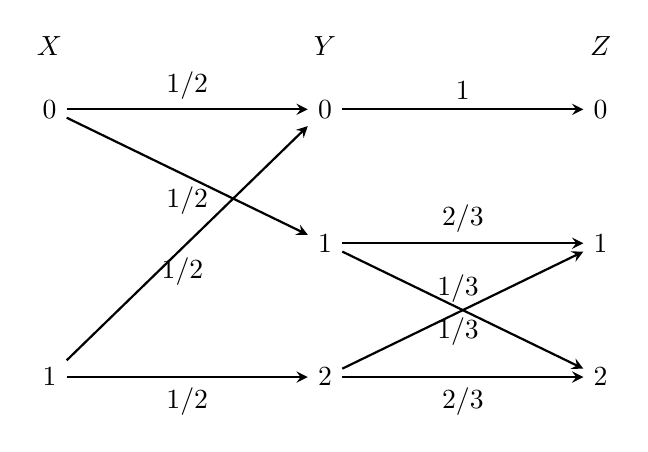
\begin{tikzpicture}[>=stealth, thick, xscale=1.0, yscale=1.0]

% X nodes
\node (x0) at (0,3.4) {$0$};
\node (x1) at (0,0) {$1$};
\node at (0,4.2) {$X$};

% Y nodes
\node (y0) at (3.5,3.4) {$0$};
\node (y1) at (3.5,1.7) {$1$};
\node (y2) at (3.5,0) {$2$};
\node at (3.5,4.2) {$Y$};

% Z nodes
\node (z0) at (7.0,3.4) {$0$};
\node (z1) at (7.0,1.7) {$1$};
\node (z2) at (7.0,0) {$2$};
\node at (7.0,4.2) {$Z$};

% X -> Y
\draw[->] (x0) -- (y0) node[midway, above] {$1/2$};
\draw[->] (x0) -- (y1) node[midway, below] {$1/2$};

\draw[->] (x1) -- (y0) node[pos=0.48, below] {$1/2$};
\draw[->] (x1) -- (y2) node[midway, below] {$1/2$};

% Y -> Z
\draw[->] (y0) -- (z0) node[midway, above] {$1$};

\draw[->] (y1) -- (z1) node[midway, above] {$2/3$};
\draw[->] (y1) -- (z2) node[pos=0.48, below] {$1/3$};

\draw[->] (y2) -- (z1) node[pos=0.48, above] {$1/3$};
\draw[->] (y2) -- (z2) node[midway, below] {$2/3$};

\end{tikzpicture}

图：级联信道
\end{center}

\begin{enumerate}[label=\arabic*., leftmargin=2em, itemsep=1.0em]

\item 求级联信道的信道容量及最佳输入概率分布。

\item 若 $X$ 信源输出两个等概消息 $S_1$ 和 $S_2$，用级联信道输入符号集中的符号对 $S_1$ 和 $S_2$ 进行信道编码：$W_1=00$ 代表 $S_1$，$W_2=11$ 代表 $S_2$。试写出在最终输出端使平均错误译码概率最小的译码规则，并计算对应的平均错误译码概率。

\end{enumerate}




\newpage

\begin{center}
{\heiti\zihao{3} 参考答案}
\end{center}

\vspace{1em}

%================================================
% 卷一
%================================================

\begin{center}
{\heiti\zihao{4} 卷一参考答案}
\end{center}

\section*{一、概念题}

\begin{enumerate}[label=\arabic*., leftmargin=2em]
\item 错误。信道疑义度 $H(X|Y)\geq 0$，但可以等于 $0$。

\item 正确。信道容量
\[
C=\max_{p(x)}I(X;Y),
\]
只由信道统计特性决定。

\item 错误。齐次性只表示转移概率不随时间变化，不能推出平稳性。

\item 正确。若信息传输速率大于信道容量，则不存在使差错率任意小的信道编码。

\item 错误。线性分组码的最小汉明距离等于所有非零码字的最小汉明重量。

\item 不是。

例如
\[
10\,110=10110,\qquad 1011\,0=10110,
\]
同一码序列有两种译法，所以不是唯一可译码。

\item 最少；减。

\item 上凸。

\item $0$；$1$。

\item $1$；$0$。
\end{enumerate}

\section*{二、信道编码题}

设
\[
C=\{11100,\ 01001,\ 10010,\ 00111\}.
\]

\begin{enumerate}[label=\arabic*., leftmargin=2em]
\item 逐对计算汉明距离：
\[
\begin{aligned}
d(11100,01001)&=3,\\
d(11100,10010)&=3,\\
d(11100,00111)&=4,\\
d(01001,10010)&=4,\\
d(01001,00111)&=3,\\
d(10010,00111)&=3.
\end{aligned}
\]
所以
\[
d_{\min}=3.
\]

\item 码字等概，共有 $4$ 个码字，每个码字携带
\[
\log_2 4=2\ \text{bit}.
\]
码长为 $5$，所以信息传输速率为
\[
R=\frac{2}{5}=0.4\ \text{bit/码元}.
\]

\item 对接收序列 $01100$：
\[
d(01100,11100)=1,
\]
所以译为
\[
11100.
\]

对接收序列 $00100$：
\[
d(00100,11100)=2,\qquad d(00100,00111)=2.
\]
距离相同，不能唯一判决，可译为
\[
11100\quad \text{或}\quad 00111.
\]

\item 因为
\[
d_{\min}=3,
\]
所以纠错能力为
\[
t=\left\lfloor\frac{d_{\min}-1}{2}\right\rfloor
=\left\lfloor\frac{3-1}{2}\right\rfloor=1.
\]
因此该码能纠正 $1$ 位码元错误。
\end{enumerate}

\section*{三、马尔可夫信源}

状态转移矩阵为
\[
P=
\begin{bmatrix}
1/3&1/3&1/3\\
1/3&1/3&1/3\\
1/2&1/2&0
\end{bmatrix}.
\]

\begin{enumerate}[label=\arabic*., leftmargin=2em]
\item 设稳态分布为
\[
\boldsymbol{\pi}=(\pi_a,\pi_b,\pi_c),
\]
则
\[
\boldsymbol{\pi}P=\boldsymbol{\pi},\qquad
\pi_a+\pi_b+\pi_c=1.
\]
解得
\[
\pi_a=\frac38,\qquad
\pi_b=\frac38,\qquad
\pi_c=\frac14.
\]

各状态条件熵为
\[
H(X_i|X_{i-1}=a)=\log_2 3,
\]
\[
H(X_i|X_{i-1}=b)=\log_2 3,
\]
\[
H(X_i|X_{i-1}=c)=1.
\]

所以信源熵为
\[
\begin{aligned}
H_\infty
&=\frac38\log_2 3+\frac38\log_2 3+\frac14\cdot 1\\
&=\frac34\log_2 3+\frac14\\
&\approx 1.439\ \text{bit/符号}.
\end{aligned}
\]

\item 符号集大小为 $3$，最大熵为
\[
H_{\max}=\log_2 3.
\]
剩余度为
\[
\begin{aligned}
R
&=1-\frac{H_\infty}{H_{\max}}\\
&=1-\frac{\frac34\log_2 3+\frac14}{\log_2 3}\\
&\approx 0.0923.
\end{aligned}
\]

\item 达到稳态时的符号概率分布为
\[
P(a)=\frac38,\qquad
P(b)=\frac38,\qquad
P(c)=\frac14.
\]
\end{enumerate}

\section*{四、离散无记忆信道}

信道矩阵为
\[
P=
\begin{bmatrix}
1/2&1/4&1/4\\
1/4&1/2&1/4
\end{bmatrix}.
\]

\begin{enumerate}[label=\arabic*., leftmargin=2em]
\item 设
\[
P(X=0)=p,\qquad P(X=1)=1-p.
\]
则输出分布为
\[
P(Y=0)=\frac14+\frac p4,
\]
\[
P(Y=1)=\frac12-\frac p4,
\]
\[
P(Y=2)=\frac14.
\]

两行条件熵相同：
\[
H(Y|X)=H\left(\frac12,\frac14,\frac14\right)=\frac32.
\]

所以
\[
I(X;Y)=H(Y)-\frac32.
\]

当
\[
P(Y=0)=P(Y=1)=\frac38
\]
时，$H(Y)$ 最大。由
\[
\frac14+\frac p4=\frac38
\]
得
\[
p=\frac12.
\]

因此最佳输入分布为
\[
P(X=0)=P(X=1)=\frac12.
\]
对应输出分布为
\[
P(Y=0)=\frac38,\qquad
P(Y=1)=\frac38,\qquad
P(Y=2)=\frac14.
\]

信道容量为
\[
\begin{aligned}
C
&=H\left(\frac38,\frac38,\frac14\right)-\frac32\\
&\approx 1.5613-1.5\\
&=0.0613\ \text{bit/符号}.
\end{aligned}
\]

\item 编码为
\[
S_1\to W_1=00,\qquad S_2\to W_2=11.
\]

由于 $S_1,S_2$ 等概，应采用最大似然译码。

译码规则为：
\[
\begin{cases}
\text{若输出序列中 }0\text{ 的个数多于 }1\text{ 的个数，则译为 }S_1,\\
\text{若输出序列中 }1\text{ 的个数多于 }0\text{ 的个数，则译为 }S_2,\\
\text{若二者个数相同，则可任意判决。}
\end{cases}
\]

平均正确译码概率为
\[
P_c=\frac12\sum_y\max\{P(y|00),P(y|11)\}
=\frac{21}{32}.
\]
所以平均错误译码概率为
\[
P_e=1-P_c=\frac{11}{32}.
\]
\end{enumerate}

\section*{五、空缺题}

原题空缺，暂无答案。

\section*{六、线性分组码}

将原生成矩阵化为系统形式：
\[
G_s=
\begin{bmatrix}
1&0&0&0&1&0&1\\
0&1&0&0&1&1&1\\
0&0&1&0&1&1&0\\
0&0&0&1&0&1&1
\end{bmatrix}
=\left[I_4\mid P\right],
\]
其中
\[
P=
\begin{bmatrix}
1&0&1\\
1&1&1\\
1&1&0\\
0&1&1
\end{bmatrix}.
\]

\begin{enumerate}[label=\arabic*., leftmargin=2em]
\item 输入序列为
\[
0101000100001110.
\]
每 $4$ 位分组：
\[
0101,\quad 0001,\quad 0000,\quad 1110.
\]

对应系统码为
\[
0101\to 0101100,
\]
\[
0001\to 0001011,
\]
\[
0000\to 0000000,
\]
\[
1110\to 1110100.
\]

所以编码输出为
\[
0101100\ 0001011\ 0000000\ 1110100.
\]

\item 监督矩阵为
\[
H=\left[P^T\mid I_3\right],
\]
即
\[
H=
\begin{bmatrix}
1&1&1&0&1&0&0\\
0&1&1&1&0&1&0\\
1&1&0&1&0&0&1
\end{bmatrix}.
\]

\item 接收码字为
\[
B=1110001.
\]
计算伴随式：
\[
S=HB^T
=
\begin{bmatrix}
1\\0\\1
\end{bmatrix}.
\]

伴随式等于 $H$ 的第 $1$ 列，因此第 $1$ 位出错。

纠错后码字为
\[
0110001.
\]
\end{enumerate}

\section*{七、循环码}

\begin{enumerate}[label=\arabic*., leftmargin=2em]
\item 取信息位为前 $3$ 位，可得标准形式生成矩阵：
\[
G=
\begin{bmatrix}
1&0&0&1&0&1&1\\
0&1&0&1&1&1&0\\
0&0&1&0&1&1&1
\end{bmatrix}
=\left[I_3\mid P\right].
\]

其中
\[
P=
\begin{bmatrix}
1&0&1&1\\
1&1&1&0\\
0&1&1&1
\end{bmatrix}.
\]

所以监督矩阵为
\[
H=\left[P^T\mid I_4\right],
\]
即
\[
H=
\begin{bmatrix}
1&1&0&1&0&0&0\\
0&1&1&0&1&0&0\\
1&1&1&0&0&1&0\\
1&0&1&0&0&0&1
\end{bmatrix}.
\]

\item 信息位为 $101$ 时，生成码字为
\[
1011100.
\]

若按从左到右对应 $x^0,x^1,\cdots,x^6$，则码多项式为
\[
c(x)=1+x^2+x^3+x^4.
\]

若按高次幂在左的习惯，则为
\[
c(x)=x^6+x^4+x^3+x^2.
\]

\item 非零码字最小重量为
\[
d_{\min}=4.
\]
所以纠错能力为
\[
t=\left\lfloor\frac{d_{\min}-1}{2}\right\rfloor
=\left\lfloor\frac{4-1}{2}\right\rfloor=1.
\]
因此该码能纠正 $1$ 位错误。
\end{enumerate}


%================================================
% 卷二
%================================================

\newpage

\begin{center}
{\heiti\zihao{4} 卷二参考答案}
\end{center}

\section*{一、空缺题}

原题空缺，暂无答案。

\section*{二、简答题}

\begin{enumerate}[label=\arabic*., leftmargin=2em]
\item 每个像素有 $256$ 个等概亮度电平，所以每个像素携带
\[
\log_2 256=8\ \text{bit}.
\]

每帧图像有 $20$ 万个像素，因此平均每帧图像携带信息量为
\[
20\times 10^4\times 8=1.6\times 10^6\ \text{bit}.
\]

每秒发送 $25$ 帧，所以信息传输速率为
\[
R=25\times 1.6\times 10^6
=4.0\times 10^7\ \text{bit/s}.
\]

信噪比为
\[
30\,\mathrm{dB},
\]
所以
\[
\frac SN=10^{30/10}=1000.
\]

由香农公式：
\[
C=B\log_2\left(1+\frac SN\right),
\]
令 $C=R$，得
\[
B=\frac{4.0\times 10^7}{\log_2 1001}
\approx 4.01\times 10^6\ \mathrm{Hz}.
\]

因此所需带宽约为
\[
4.01\ \mathrm{MHz}.
\]

\item 费诺不等式为
\[
H(X|Y)\leq H(P_E)+P_E\log(r-1).
\]

其物理意义是：译码错误概率越小，接收端对发送符号的不确定性越小；若信道疑义度 $H(X|Y)$ 较大，则错误译码概率不可能任意小。
\end{enumerate}

\section*{三、空缺题}

原题空缺，暂无答案。

\section*{四、空缺题}

原题空缺，暂无答案。

\section*{五、空缺题}

原题空缺，暂无答案。

\section*{六、级联信道}

单个信道的转移矩阵为
\[
P=
\begin{bmatrix}
1&0\\
1/2&1/2
\end{bmatrix}.
\]

两个信道级联后：
\[
P^2=
\begin{bmatrix}
1&0\\
3/4&1/4
\end{bmatrix}.
\]

\begin{enumerate}[label=\arabic*., leftmargin=2em]
\item 已知输入等概：
\[
P(X=0)=P(X=1)=\frac12.
\]

输出分布为
\[
P(Z=0)=\frac12\cdot 1+\frac12\cdot \frac34=\frac78,
\]
\[
P(Z=1)=\frac18.
\]

所以
\[
H(Z)=H\left(\frac18\right)\approx 0.5436.
\]

又因为
\[
H(Z|X=0)=0,
\]
\[
H(Z|X=1)=H\left(\frac14\right)\approx 0.8113,
\]
所以
\[
H(Z|X)=\frac12\cdot 0+\frac12\cdot 0.8113
\approx 0.4056.
\]

因此
\[
I(X;Z)=H(Z)-H(Z|X)
\approx 0.5436-0.4056
=0.1379\ \text{bit/符号}.
\]

\item 该级联信道每秒传输 $1000$ 个输入符号，$10$ 秒共传输
\[
1000\times 10=10000
\]
个输入符号。

由于输入等概，$10000$ 个二元符号所含信息量为
\[
10000\ \text{bit}.
\]

但级联信道实际传送的信息量为
\[
10000\times 0.1379\approx 1379\ \text{bit}.
\]

因此 $10$ 秒钟不能将 $10000$ 个二元符号所含的信息量全部传送完。

\item 重复编码为
\[
0\to W_1=000,\qquad 1\to W_2=111.
\]

对于级联信道：
\[
P(Z=1|X=0)=0,\qquad P(Z=1|X=1)=\frac14.
\]

译码规则为：
\[
\begin{cases}
\text{若输出序列中至少出现一个 }1,\text{ 则译为 }1,\\
\text{若输出序列为 }000,\text{ 则译为 }0.
\end{cases}
\]

错误只会发生在发送 $111$，但输出为 $000$ 时：
\[
P_e=\frac12\left(\frac34\right)^3
=\frac{27}{128}.
\]

\item 对 $n$ 个信道级联，有
\[
P^n=
\begin{bmatrix}
1&0\\
1-2^{-n}&2^{-n}
\end{bmatrix}.
\]

当
\[
n\to\infty
\]
时，
\[
P^n\to
\begin{bmatrix}
1&0\\
1&0
\end{bmatrix}.
\]

此时输出与输入无关，所以信道容量为
\[
C=0.
\]
\end{enumerate}


%================================================
% 卷三
%================================================

\newpage

\begin{center}
{\heiti\zihao{4} 卷三参考答案}
\end{center}

\section*{客观题答案}

\[
1.\ C \qquad
2.\ D \qquad
3.\ ABCD \qquad
4.\ B \qquad
5.\ A
\]

\[
6.\ C \qquad
7.\ A \qquad
8.\ A \qquad
9.\ B \qquad
10.\ BCD
\]

\[
11.\ B \qquad
12.\ A \qquad
13.\ A \qquad
14.\ A \qquad
15.\ B
\]

\[
16\text{--}20.\ \text{题目空缺，暂无答案。}
\]

\section*{部分题目简要说明}

\begin{enumerate}[label=\arabic*., leftmargin=2em]
\item 对于 $(n,k)$ 线性分组码，伴随式数目为
\[
2^{n-k}.
\]
若能纠正 $u$ 位及以下错误，则应满足
\[
2^{n-k}\geq \sum_{i=0}^{u}C_n^i.
\]

\item $(n,k)$ 循环码的非全零码字中，连 $0$ 的个数最多为
\[
k-1.
\]

\item 信道编码通过增加冗余，使码符号之间具有相关性，从而实现检错和纠错。信道译码与信道编码规则匹配。增加冗余会降低有效性。

\item 有噪无损信道满足
\[
H(X|Y)=0,
\]
因此可以由输出唯一确定输入。

\item 错误译码概率既与信道统计特性有关，也与译码规则有关。

\item 维拉图中
\[
H(Y|X)
\]
表示右边圆中不与左边圆相交的部分。

\item 噪声熵为
\[
H(Y|X).
\]

\item 离散信道的所有概率关系可由输入分布
\[
p(x_i)
\]
和信道转移概率
\[
p(y_j|x_i)
\]
推出。

\item 对于马尔可夫链
\[
X\to Y\to Z,
\]
有
\[
I(XY;Z)=I(Y;Z),
\]
\[
I(X;Z)\leq I(Y;Z),
\]
\[
P_{Z|X}=P_{Y|X}P_{Z|Y}.
\]

\item 单个符号互信息满足
\[
I(x_i;y_j)=I(x_i)-I(x_i|y_j)
=I(y_j)-I(y_j|x_i).
\]
所以错误选项为 B、C、D。

\item 离散信源有 $16$ 个符号，最大熵为
\[
H_{\max}=\log_2 16=4\ \text{bit/符号}.
\]

\item 条件熵应为
\[
H(Y|X)=-\sum_i\sum_j p(x_i y_j)\log p(y_j|x_i).
\]
选项 A 少乘了 $p(x_i)$，因此错误。

\item 各维联合概率分布均与时间起点无关的信源称为平稳离散信源。

\item 时齐马尔可夫信源只说明转移概率不随时间变化，极限熵是否存在还需要考虑遍历性条件。

\item
\[
I(X;X)=H(X),
\]
一般不为 $0$，所以原命题错误。
\end{enumerate}


%================================================
% 卷四
%================================================

\newpage

\begin{center}
{\heiti\zihao{4} 卷四参考答案}
\end{center}

\section*{一、判断与简答题}

\begin{enumerate}[label=\arabic*., leftmargin=2em]
\item 原题空缺，暂无答案。

\item 错误。齐次马尔可夫信源只表示转移概率不随时间变化，并不代表无论初始概率分布如何最终都会达到平稳。

应改为：满足遍历性条件的齐次马尔可夫信源，经过足够长时间后，其状态分布趋于平稳分布。

\item 正确。

由互信息链式法则：
\[
I(X_1X_2\cdots X_N;Y)
=\sum_{i=1}^{N}I(X_i;Y|X_1X_2\cdots X_{i-1}).
\]

其含义是：整个序列 $X_1X_2\cdots X_N$ 与 $Y$ 的互信息，可以分解为每个符号在已知前面符号条件下对 $Y$ 提供的新增信息量之和。

\item 固定信道转移概率时，平均互信息
\[
I(X;Y)
\]
是输入概率分布 $p(x)$ 的上凸函数。

以二进制对称信道为例，设交叉概率为 $p$，则
\[
C=1-H(p).
\]
当输入等概时，输出熵最大，平均互信息达到最大值。

其物理意义是：在固定信道条件下，选择合适的输入分布可以提高平均互信息。

\item 数据处理定理：若
\[
X\to Y\to Z
\]
构成马尔可夫链，则
\[
I(X;Z)\leq I(X;Y).
\]

也就是说，对数据进行后续处理不会增加其关于原始信源的信息量，只可能保持或减少信息量。

因此要获得更多关于源数据的信息，应在采集、观测和传输阶段减少噪声与失真，而不能指望后处理凭空增加信息。

\item 香农第二定理指出：当信息传输率小于信道容量时，存在编码方法使译码错误概率任意小。

其中，“高效率”是指信息传输速率尽量接近信道容量；

“高可靠性”是指译码错误概率可以任意小；

存在这种信道编码的必要条件是
\[
R<C.
\]
\end{enumerate}

\section*{二、两个实验观察信源}

信源分布为
\[
P(0)=\frac14,\qquad P(1)=\frac14,\qquad P(2)=\frac12.
\]

\begin{enumerate}[label=\arabic*., leftmargin=2em]
\item 先求 $I(X;Y_1)$。

由表可得
\[
P(Y_1=0)=\frac14+\frac12\cdot\frac12=\frac12,
\]
\[
P(Y_1=1)=\frac12.
\]
所以
\[
H(Y_1)=1.
\]

又因为
\[
H(Y_1|X=0)=0,\qquad H(Y_1|X=1)=0,\qquad H(Y_1|X=2)=1,
\]
所以
\[
H(Y_1|X)=\frac12.
\]

因此
\[
I(X;Y_1)=H(Y_1)-H(Y_1|X)
=1-\frac12=\frac12.
\]

再求 $I(X;Y_2)$。

由表可知，$Y_2$ 是 $X$ 的确定函数，所以
\[
H(Y_2|X)=0.
\]

又
\[
P(Y_2=0)=P(X=0)+P(X=1)=\frac12,
\]
\[
P(Y_2=1)=P(X=2)=\frac12.
\]
因此
\[
H(Y_2)=1.
\]

所以
\[
I(X;Y_2)=H(Y_2)-H(Y_2|X)=1.
\]

因为
\[
I(X;Y_2)>I(X;Y_1),
\]
所以第二个实验更好。

\item 联合观察 $(Y_1,Y_2)$ 可以唯一确定 $X$，所以
\[
H(X|Y_1Y_2)=0.
\]

信源熵为
\[
\begin{aligned}
H(X)
&=-\frac14\log_2\frac14-\frac14\log_2\frac14-\frac12\log_2\frac12\\
&=\frac32.
\end{aligned}
\]

因此
\[
I(X;Y_1Y_2)=H(X)-H(X|Y_1Y_2)=\frac32.
\]

又因为
\[
I(X;Y_1Y_2)=I(X;Y_1)+I(X;Y_2|Y_1),
\]
所以
\[
I(X;Y_2|Y_1)=\frac32-\frac12=1.
\]

其中，$I(X;Y_1Y_2)$ 表示两个实验联合后获得的关于 $X$ 的信息量；
$I(X;Y_2|Y_1)$ 表示已知 $Y_1$ 后，$Y_2$ 还能额外提供的信息量。
\end{enumerate}

\section*{三、二进制数据序列}

\begin{enumerate}[label=\arabic*., leftmargin=2em]
\item 若符号之间没有关联，则
\[
H(X)=-0.45\log_2 0.45-0.55\log_2 0.55.
\]
计算得
\[
H(X)\approx 0.993\ \text{bit/符号}.
\]

\item 将二阶马尔可夫信源的状态记为
\[
00,\ 01,\ 10,\ 11.
\]

状态转移矩阵为
\[
P=
\begin{bmatrix}
1/2&1/2&0&0\\
0&0&4/5&1/5\\
1/5&4/5&0&0\\
0&0&1/2&1/2
\end{bmatrix}.
\]

设稳态分布为
\[
\boldsymbol{\pi}=(\pi_{00},\pi_{01},\pi_{10},\pi_{11}),
\]
由
\[
\boldsymbol{\pi}P=\boldsymbol{\pi}
\]
解得
\[
\pi_{00}=\frac17,\qquad
\pi_{01}=\frac{5}{14},\qquad
\pi_{10}=\frac{5}{14},\qquad
\pi_{11}=\frac17.
\]

各状态条件熵为
\[
H(X|00)=1,
\]
\[
H(X|01)=H(0.8,0.2),
\]
\[
H(X|10)=H(0.2,0.8),
\]
\[
H(X|11)=1.
\]

其中
\[
H(0.8,0.2)\approx 0.7219.
\]

所以
\[
\begin{aligned}
H_\infty
&=\frac17\cdot 1+\frac{5}{14}\cdot 0.7219
+\frac{5}{14}\cdot 0.7219+\frac17\cdot 1\\
&\approx 0.8014\ \text{bit/符号}.
\end{aligned}
\]

稳态下符号 $0$ 的概率为
\[
P(0)=\pi_{00}+\pi_{10}
=\frac17+\frac{5}{14}
=\frac12.
\]

因此长度为 $N$ 的序列中大约有
\[
\frac N2
\]
个 $0$。

\item 二进制信源最大熵为
\[
H_{\max}=1.
\]

第（1）问剩余度为
\[
R_1=1-H(X)\approx 1-0.993=0.007.
\]

第（2）问剩余度为
\[
R_2=1-H_\infty\approx 1-0.8014=0.1986.
\]

所以
\[
R_2>R_1.
\]

这说明考虑符号相关性后，信源不确定性降低，冗余度增加，压缩空间更大。
\end{enumerate}

\section*{四、最佳编码与费用比较}

概率分布为
\[
0.25,\ 0.25,\ 0.20,\ 0.15,\ 0.10,\ 0.05.
\]

信源熵为
\[
H(X)=-\sum_i p_i\log_2 p_i
\approx 2.4232\ \text{bit/符号}.
\]

\begin{enumerate}[label=\arabic*., leftmargin=2em]
\item 二进制最佳编码平均码长为
\[
\bar{L}_2=2.45.
\]
编码效率为
\[
\eta_2=\frac{H(X)}{\bar{L}_2}
=\frac{2.4232}{2.45}
\approx 0.989.
\]

三元最佳编码平均码长为
\[
\bar{L}_3=1.65.
\]
编码效率为
\[
\eta_3=\frac{H(X)}{\bar{L}_3\log_2 3}
=\frac{2.4232}{1.65\log_2 3}
\approx 0.927.
\]

\item 二进制编码平均费用为
\[
2.45\times 2.2=5.39\ \text{元/信源符号}.
\]

三元编码平均费用为
\[
1.65\times 3=4.95\ \text{元/信源符号}.
\]

因为
\[
4.95<5.39,
\]
所以三元编码服务更省钱。

虽然三元编码效率略低，但平均码长更短，因此总费用更低。
\end{enumerate}

\section*{五、级联信道}

由图可得第一级信道为
\[
P_{Y|X}=
\begin{bmatrix}
1/2&1/2&0\\
1/2&0&1/2
\end{bmatrix}.
\]

第二级信道为
\[
P_{Z|Y}=
\begin{bmatrix}
1&0&0\\
0&2/3&1/3\\
0&1/3&2/3
\end{bmatrix}.
\]

所以级联信道为
\[
P_{Z|X}=P_{Y|X}P_{Z|Y}.
\]

计算得
\[
P_{Z|X}=
\begin{bmatrix}
1/2&1/3&1/6\\
1/2&1/6&1/3
\end{bmatrix}.
\]

\begin{enumerate}[label=\arabic*., leftmargin=2em]
\item 设
\[
P(X=0)=p,\qquad P(X=1)=1-p.
\]

输出分布为
\[
P(Z=0)=\frac12,
\]
\[
P(Z=1)=\frac16+\frac p6,
\]
\[
P(Z=2)=\frac13-\frac p6.
\]

两行条件熵相同：
\[
H(Z|X)=H\left(\frac12,\frac13,\frac16\right).
\]

因此
\[
I(X;Z)=H(Z)-H(Z|X).
\]

当
\[
P(Z=1)=P(Z=2)=\frac14
\]
时，$H(Z)$ 最大。由
\[
\frac16+\frac p6=\frac14
\]
得
\[
p=\frac12.
\]

所以最佳输入分布为
\[
P(X=0)=P(X=1)=\frac12.
\]

此时输出分布为
\[
P(Z=0)=\frac12,\qquad
P(Z=1)=\frac14,\qquad
P(Z=2)=\frac14.
\]

信道容量为
\[
\begin{aligned}
C
&=H\left(\frac12,\frac14,\frac14\right)
-H\left(\frac12,\frac13,\frac16\right)\\
&\approx 1.5-1.4591\\
&=0.0409\ \text{bit/符号}.
\end{aligned}
\]

\item 编码规则为
\[
S_1\to W_1=00,\qquad S_2\to W_2=11.
\]

由于 $S_1,S_2$ 等概，应采用最大似然译码。

单个输出符号中，$1$ 更支持输入 $0$，$2$ 更支持输入 $1$，$0$ 对二者支持相同。

译码规则为：
\[
\begin{cases}
\text{若输出序列中 }1\text{ 的个数多于 }2\text{ 的个数，则译为 }S_1,\\
\text{若输出序列中 }2\text{ 的个数多于 }1\text{ 的个数，则译为 }S_2,\\
\text{若二者个数相同，则可任意判决。}
\end{cases}
\]

平均正确译码概率为
\[
P_c=\frac12\sum_z\max\{P(z|00),P(z|11)\}
=\frac58.
\]

所以平均错误译码概率为
\[
P_e=1-P_c=\frac38.
\]
\end{enumerate}

\end{document}
